\begin{frame}
  \frametitle{これからやること}
  \begin{itemize}
    \item LEDを使ったプログラムの復習
    \item 新しいセンサーを使ったプログラム
    \item 複数のセンサーを使ったプログラム
  \end{itemize}
\end{frame}

\begin{frame}
  \frametitle{センサーボードってなんだろう}
  \begin{columns}
    \begin{column}{0.48\textwidth}
      \begin{itemize}
        \item 4色のLED
        \item 照度センサー
        \item 赤外線LED
        \item 赤外線受信ユニット
        \item 温湿度気圧センサー
      \end{itemize}
    \end{column}
    \begin{column}{0.48\textwidth}
      \begin{figure}
        \centering

        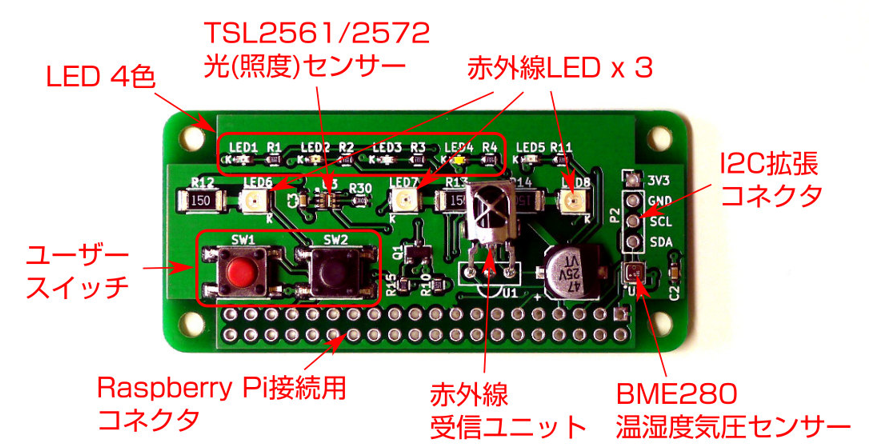
\includegraphics[width=1.0\textwidth]{../images/chap03/sensors_name.png}
        \caption{センサーボード}
      \end{figure}
    \end{column}
  \end{columns}
\end{frame}

\begin{frame}
  \frametitle{センサーボードを取り付けよう}
  \begin{figure}
    \centering

    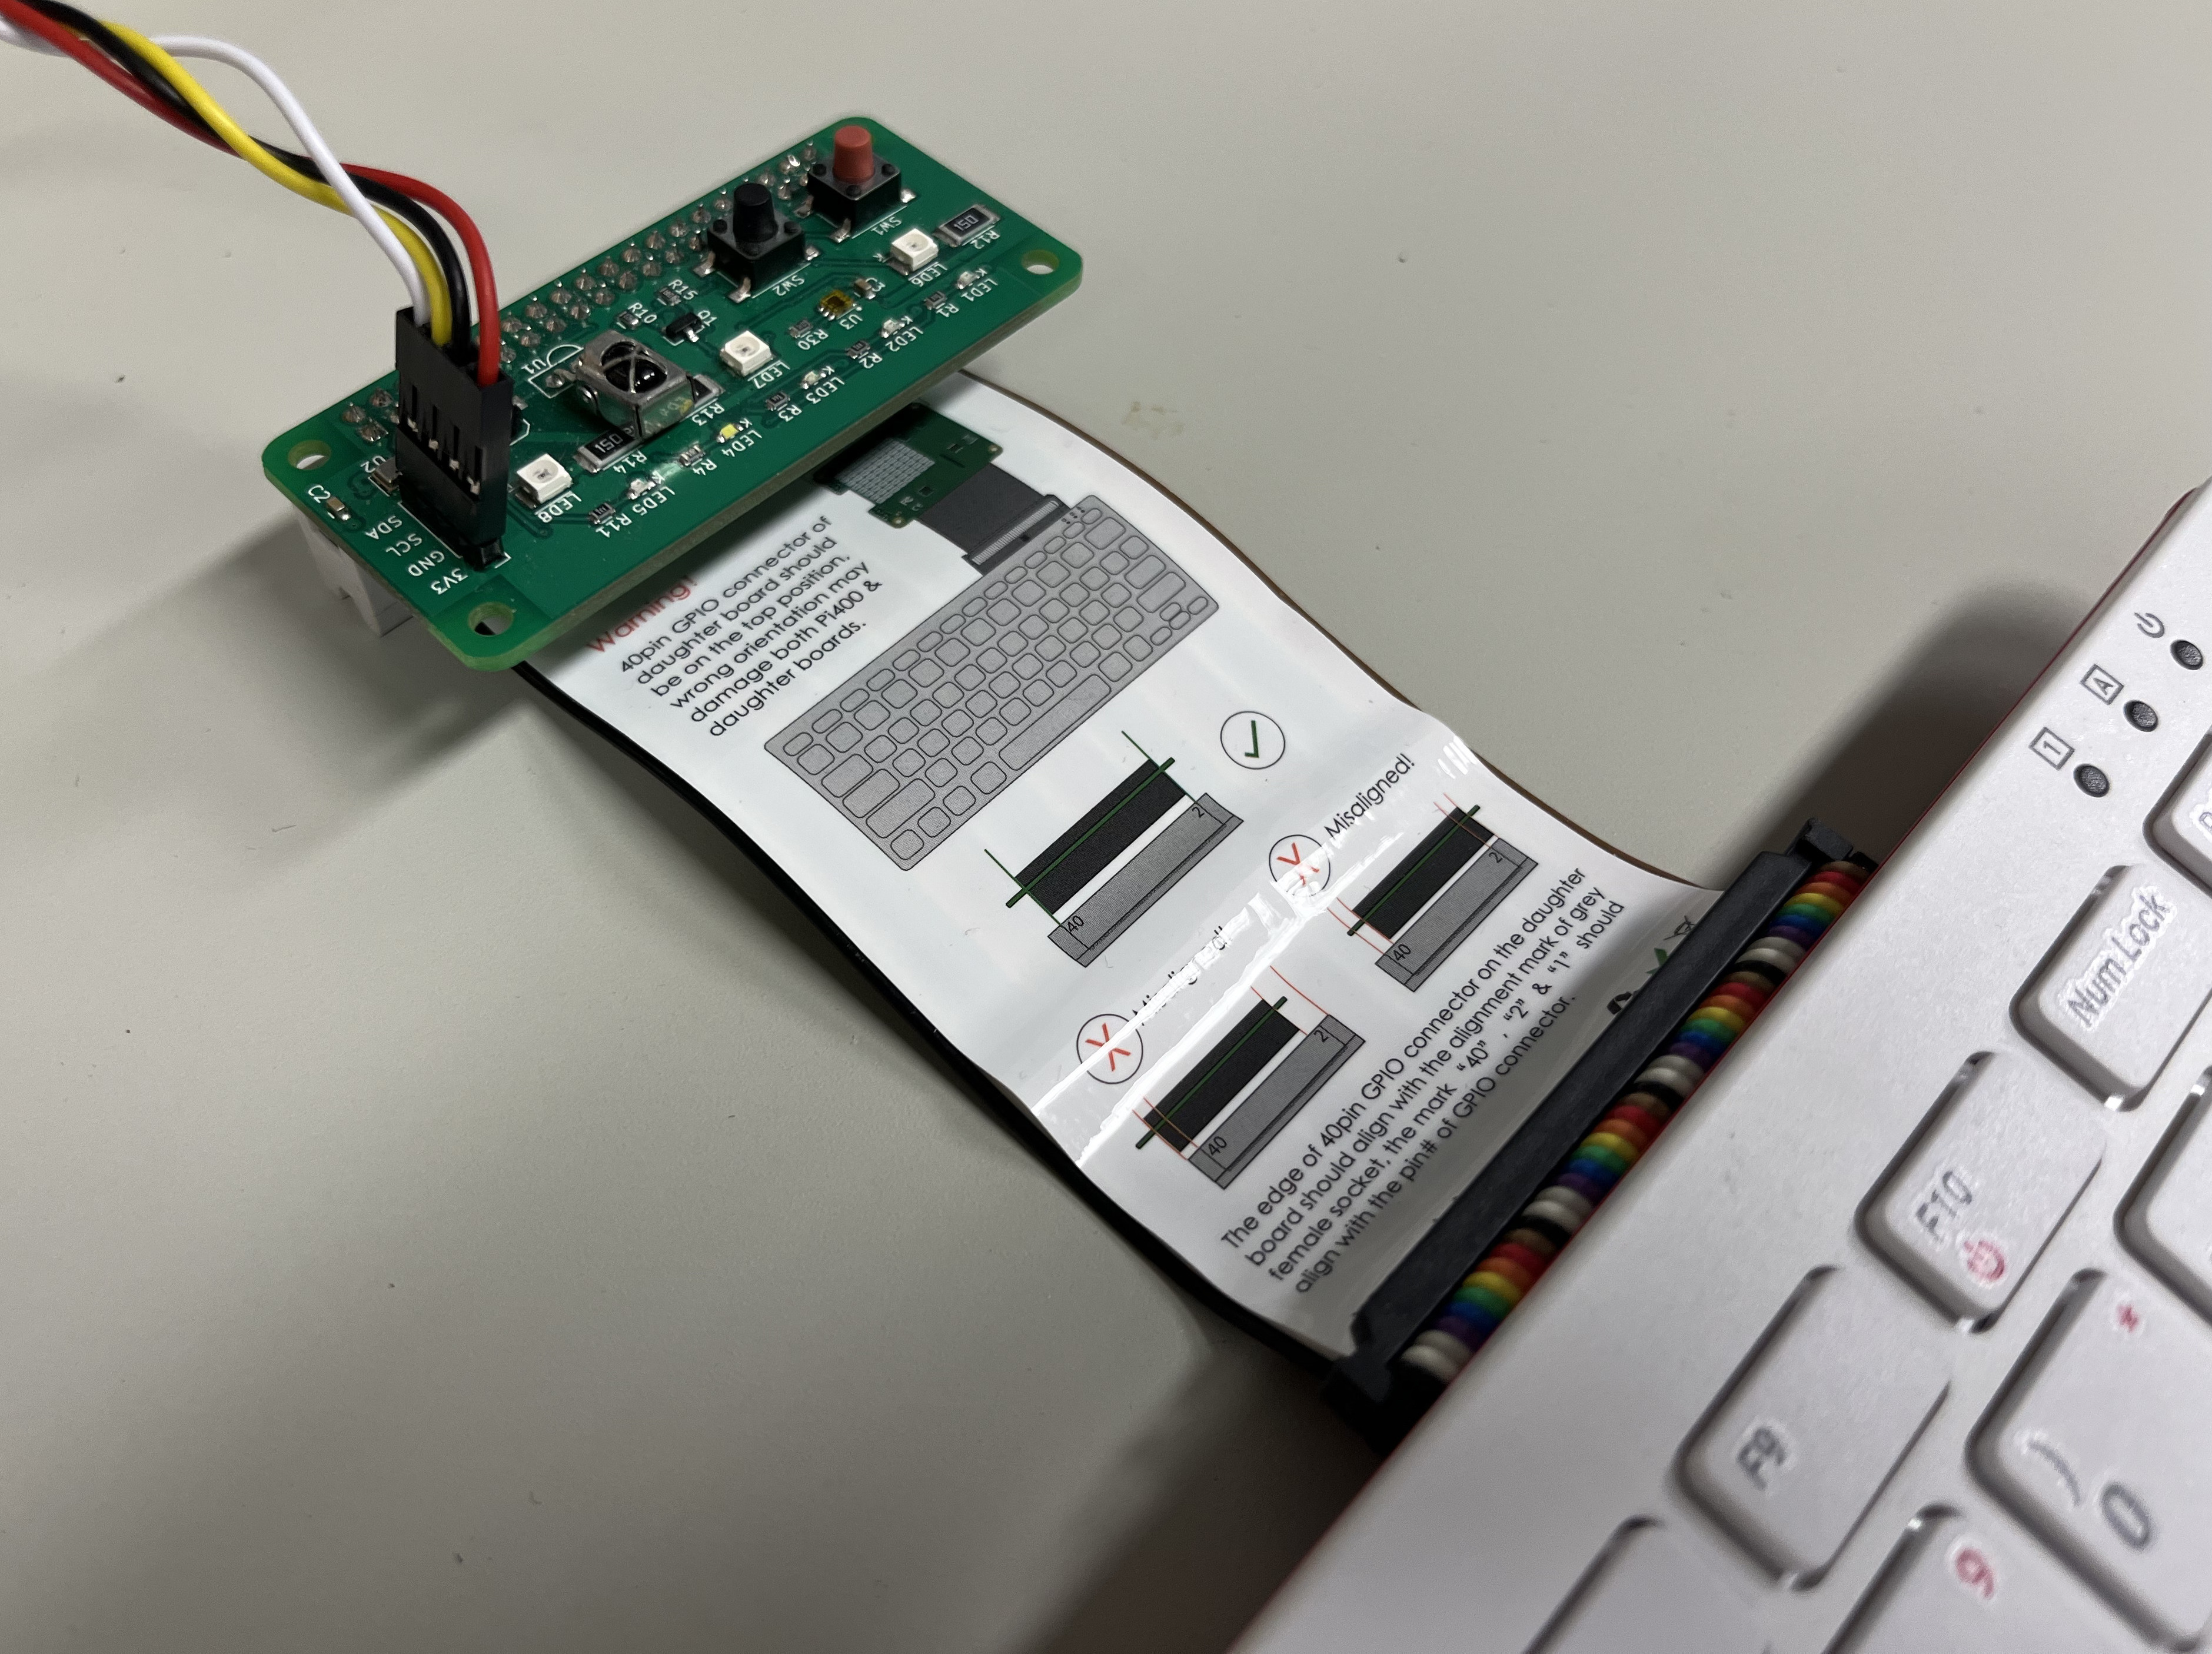
\includegraphics[width=0.5\textwidth]{../images/chap03/how_to_install_bme280.jpg}
    \caption{外付けのセンサー}
  \end{figure}
  \begin{itemize}
    \item 一度シャットダウンしてからセンサーボードを差し込む
    \item 赤色の線が3V3に来るようにする
  \end{itemize}
\end{frame}

\begin{frame}
  \frametitle{LEDを光らせよう(1)}
  \begin{itemize}
    \item led.hspを実行しよう
    \begin{itemize}
      \item ターミナルでhsedコマンドを使おう
      \item ファイル\rightarrow 開く\rightarrow led.hsp
    \end{itemize}
  \end{itemize}
\end{frame}

\begin{frame}[fragile]
  \frametitle{LEDを光らせてみよう(2)}
  \begin{lstlisting}[title=led.hsp,label=led.hsp]
  #include "hsp3dish.as"   <#blue#;スクリプトの設定を読み込む#>
  #include "rpz-gpio.as"   <#blue#;スクリプトの設定を読み込む#>
          redraw 0         <#blue#;画面更新 (仮想画面に描画)#>
          font "",30       <#blue#;文字のフォント、サイズを決める#>
          pos 20, 20       <#blue#;文字の場所を決める#>
          mes "LEDが光るよ" <#blue#;文字を決める#>
          redraw 1         <#blue#;画面更新(実際の画面に描画)#>
  *led
          gpio 17, 1     <#blue#;GPIO17を点灯させる#>
          wait 100       <#blue#;0.1 秒待つ#>
          goto *led      <#blue#;*led まで戻る#>
          gpio 17, 0     <#blue#;GPIO17を消灯させる#>
  \end{lstlisting}
\end{frame}

\begin{frame}
  \frametitle{LEDを光らせてみよう(3)}
  \begin{itemize}
    \item gpio 17, 1 の部分でLEDを光らせているよ
          \begin{itemize}
            \item 17 は光らせたいLEDのGPIO番号
            \item 1で点灯、0で消灯
          \end{itemize}
  \end{itemize}
\end{frame}

\begin{frame}
  \frametitle{問題をといてみよう!}
  \begin{itemize}
    \item 教科書28ページ 問題3-7(4問)
  \end{itemize}
\end{frame}

\begin{frame}
  \frametitle{温度、湿度、気圧、明るさを調べてみよう(1)}
  \begin{itemize}
    \item sensors.hspを実行しよう
  \end{itemize}
\end{frame}

\begin{frame}[fragile]
  \frametitle{温度、湿度、気圧、明るさを調べてみよう(2)}
  \begin{lstlisting}[title=sensors.hsp, label=sensors.hsp]
   #include "hsp3dish.as"    
   #include "jtalk.as"    

   init_bme               <#blue#; 温湿度気圧センサ#>
   if stat {              <#blue#; 初期化成功チェック#>
     redraw 0          
     mes "failed to init bme: " + stat
     redraw 1
     stop
   }

   geti2c_lux_init     <#blue#; 照度センサ tsl2572 を初期化する#>

   *main
   redraw 0            <#blue#; 仮想画面に描画#>
   pos 60, 60          <#blue#; 表示位置を設定#>
  
  \end{lstlisting}
\end{frame}

\begin{frame}[fragile]
  \frametitle{温度、湿度、気圧、明るさを調べてみよう(2)(コード続き)}
  \begin{lstlisting}[title=sensors.hsp, label=sensors.hsp]
  get_humidity          <#blue#; rpz_humに湿度取得#>
  hum = rpz_hum       
  get_pressure          <#blue#; rpz_pressに気圧取得#>
  press = rpz_press
  geti2_lux_als         <#blue#; rpz_luxに照度取得#>
  lux = rpz_lux
  mes "温度: " + temp + " [℃]" <#blue#; 取得したデータの表示#>
  mes "湿度: " + hum + " [%]"
  mes "気圧: " + press + "[hPa]"
  mes "照度: " + lux + " [lx]"
  redraw 1              
  wait 100
  goto *main
  \end{lstlisting}
\end{frame}

\begin{frame}
  \frametitle{問題をといてみよう!}
  \begin{itemize}
    \item 教科書32ページ 問題3-9(8問)
  \end{itemize}
\end{frame}

\begin{frame}
  \frametitle{ボタンを使ってLEDをつけてみよう(1)}
    \begin{itemize}
    \item button\_led.hspを実行しよう
  \end{itemize}
\end{frame}

\begin{frame}[fragile]
  \frametitle{ボタンを使ってLEDをつけてみよう(2)}
  \begin{lstlisting}[title=button\_led.hsp, label=button_led.hsp]
  #include "hsp3dish.as"
  #include "rpz-gpio.as"
  
          gpio 17, 0
          gpio 18, 0
          gpio 22, 0
          gpio 27, 0

          redraw 0
          font "", 30
          pos 20, 20
          mes "ボタンを押している間 LED が光るよ"
          redraw 1
  *led
          bnt1 = gpioin(5)        <#blue#;ボタンの状態を調べる#>
          if btn1=0 : gpio 18, 1  <#blue#;ボタンによってLEDを点灯/消灯#>
          wait 10                 <#blue#;0.1秒待つ#>
          goto *led               <#blue#;*ledに戻る#>
  \end{lstlisting}
\end{frame}

\begin{frame}
  \frametitle{ボタンが押されているか調べる命令}
  \begin{itemize}
    \item gpioin()
          \begin{itemize}
            \item ()の中にはGPIO番号が入るよ
            \item 赤ボタンならGPIO=5、黒ボタンならGPIO=6
          \end{itemize}
    \item ima\_btn = gpioin(5)
          \begin{itemize}
            \item GPIO5(赤ボタン)が押されたかどうかを数字で判定
            \item 押されたらima\_btn=0、はなされたらima\_btn=1
          \end{itemize}
  \end{itemize}
\end{frame}

\begin{frame}
  \frametitle{問題をといてみよう!}
  \begin{itemize}
    \item 教科書34ページ 問題3-10(3問)
  \end{itemize}
\end{frame}

\begin{frame}
  \frametitle{ボタンを使ってLEDをつけてみよう(3)}
    \begin{itemize}
    \item button\_led2.hspを実行しよう
  \end{itemize}
\end{frame}

\begin{frame}[fragile]
  \frametitle{ボタンを使ってLEDをつけてみよう(4)}
  \begin{lstlisting}[title=button\_led2.hsp, label=button_led2.hsp]
  #include "hsp3dish.as"
  #include "rpz-gpio.as"
  
          gpio 17, 0
          gpio 18, 0
          gpio 22, 0
          gpio 27, 0
        
          redraw 0
          font "", 30
          pos 20, 20
          mes "赤いボタンを押して、LED をつけたり消したりできるよ"
          redraw 1

          ima_btn = 1   <#blue#;今ボタンを押しているかどうかの変数#>
          mae_btn = 1   <#blue#;前回はボタンを押しているかどうかの変数#>
          led = 1       <#blue#;LEDを光らせるか決める変数#>
  \end{lstlisting}
\end{frame}

\begin{frame}[fragile]
  \frametitle{ボタンを使ってLEDをつけてみよう(4) (コード続き)}
  \begin{lstlisting}[title=button\_led2.hsp, label=button_led2.hsp]
  *hata
          ima_btn = gpioin(5)
          if ima_btn = 0{    <#blue#;今押されているとき#>
            if mae_btn = 1{  <#blue#;前は押されていなかった時#>
              led = 1 - led  <#blue#;LEDの消灯を切り替える#>
            }
          }

          gpio 22, led       <#blue#;GPIO22をつけるか消すかする#>
          mae_btn = ima_btn  <#blue#;今の状態を前回の状態とする#>

          wait 10
          goto *hata
  \end{lstlisting}
\end{frame}

\begin{frame}
  \frametitle{ボタンを押してLEDをon/offするには}
  \begin{itemize}
    \item ボタンを押したかどうやってわかるの?
  \end{itemize}
  \begin{figure}
    \centering
    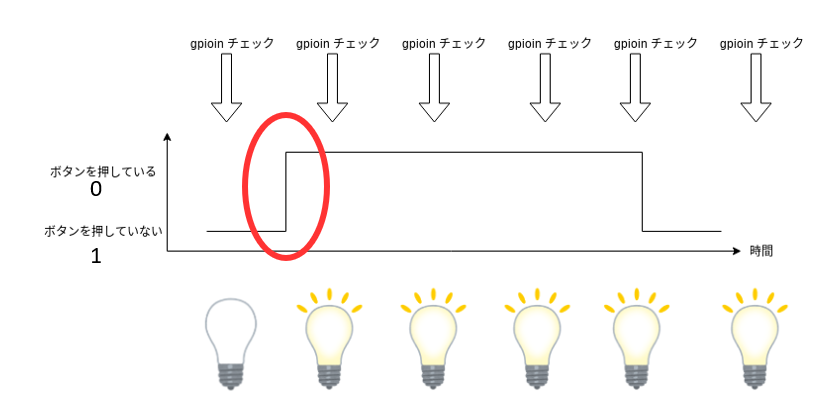
\includegraphics[width=0.8\textwidth]{../images/chap03/button_push.png}
  \end{figure}
\end{frame}

\begin{frame}
  \frametitle{問題をといてみよう!}
  \begin{itemize}
    \item 教科書36ページ 問題3-11(4問)
  \end{itemize}
\end{frame}

\begin{frame}
  \frametitle{ボタンを使ってLEDをつけてみよう(5)}
    \begin{itemize}
    \item button\_led3.hspを実行しよう
  \end{itemize}
\end{frame}

\begin{frame}[fragile]
  \frametitle{ボタンを使ってLEDをつけてみよう(6)}
  \begin{lstlisting}[title=button\_led3.hsp, label=button_led3.hsp]
  #include "hsp3dish.as"
  #include "rpz-gpio.as"
  
          gpio 17, 0   
          gpio 18, 0
          gpio 22, 0
          gpio 27, 0

          redraw 0
          font "", 30
          pos 20, 20
          mes "赤いボタンを押して、LED をつけたり消したりできるよ"
          redraw 1

          ima_btn = 1 
          ledidx = 0
  \end{lstlisting}
\end{frame}

\begin{frame}[fragile]
  \frametitle{ボタンを使ってLEDをつけてみよう(6) (コード続き)}
  \begin{lstlisting}[title=button\_led3.hsp, label=button_led3.hsp]
  *hata
          ima_btn = gpioin(5)
          if ima_btn = 0{           <#blue#;今押されているとき#>
           iedidx = (ledidx+1) \ 4  <#blue#;ledidxで何番目のLEDを光らせるか決める#>
           if ledidx=1 {            <#blue#;1番目の時はGPIO17のLEDを光らせる#>
             gpio 17, 1             <#blue#;(0+1)\4 = 1#>
             gpio 18, 0 
             gpio 22, 0
             gpio 27, 0
           }

           else : if ledidx=2 {     <#blue#;2番目の時はGPIO18のLEDを光らせる#>
             gpio 17, 0             <#blue#;(1+1)\4 = 2#>
             gpio 18, 1
             gpio 22, 0
             gpio 27, 0
           }
  \end{lstlisting}
\end{frame}

\begin{frame}[fragile]
  \frametitle{ボタンを使ってLEDをつけてみよう(6) (コード続き)}
  \begin{lstlisting}[title=button\_led3.hsp, label=button_led3.hsp]
           else : if ledidx=3{      <#blue#;3番目の時はGPIO22のLEDを光らせる#>
             gpio 17, 0             <#blue#;(2+1)\4 = 3#>
             gpio 18, 0
             gpio 22, 1
             gpio 27, 0
           }

           else : if ledidx=0 {     <#blue#;4番目の時はGPIO27のLEDを光らせる#>
             gpio 17, 0             <#blue#;(3+1)\4 = 0#>
             gpio 18, 0
             gpio 22, 0
             gpio 27, 1
           }
          }

          wait 10
          goto *hata
  \end{lstlisting}
\end{frame}

\begin{frame}
  \frametitle{LEDを右に動くようにするには?}
  \begin{itemize}
    \item ボタンを押したかどうか調べる
    \item ボタンを押した回数を調べる
    \item 何回目に押されたかで光るLEDを変える
  \end{itemize}
\end{frame}

\begin{frame}
  \frametitle{問題をといてみよう!}
  \begin{itemize}
    \item 教科書38ページ 問題3-12(3問)
  \end{itemize}
\end{frame}

\begin{frame}
  \frametitle{チャレンジ問題を解いてみよう}
  \begin{itemize}
    \item 教科書39ページ 闇夜を照らすLED
    \item 教科書40ページ GIFアニメーションの作成
  \end{itemize}
\end{frame}